\documentclass{../../../oss-ap12ibhl}

\begin{document}
\genheader
\gentitle{14}{MAGNETISM}

\begin{questions}
  \question An electron is moving downward toward the bottom of the page when
  it passes through a region of magnetic field, as shown in the figure by the
  shaded area. The electron travels along a path that takes it through the spot
  marked $X$. The gravitational force on the electron is very small. What is
  the direction of the magnetic field?

  \begin{minipage}{.2\linewidth}
    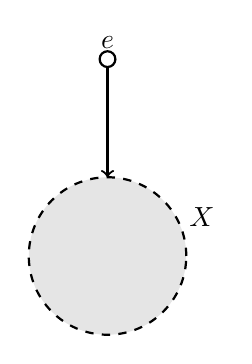
\begin{tikzpicture}
      \draw[thick,dashed,fill=gray!20](0,0) circle(1);
      \node at (1.2,.5) {$X$};
      \draw[thick](0,2.5) circle(.1) node[above]{$e$};
        \draw[thick,->](0,2.4)--(0,1);
    \end{tikzpicture}
  \end{minipage}
  \begin{minipage}{.4\linewidth}
    \begin{choices}
      \choice Toward the bottom of the page
      \choice Toward the top of the page
      \choice Out of the page
      \choice Into the page
    \end{choices}
  \end{minipage}

    
  \question Two long parallel wires carry currents ($I_A$ and $I_B$), as shown
  in the figure. Current $I_A$ in the left wire is twice that of current $I_B$
  in the right wire. The magnetic force on the right wire is $F$. What is the
  magnetic force on the left wire in terms of $F$?

  \begin{minipage}{.2\linewidth}
    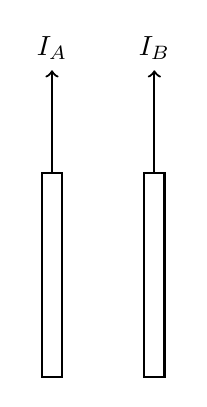
\begin{tikzpicture}[scale=1.3]
      \begin{scope}[thick]
        \draw(0,0) rectangle(.2,2);
          \draw(1,0) rectangle(1.2,2);
          \draw[->](.1,2)--(.1,3) node[above]{$I_A$};
          \draw[->](1.1,2)--(1.1,3) node[above]{$I_B$};
      \end{scope}
      \end{tikzpicture}
  \end{minipage}
  \begin{minipage}{.4\linewidth}
    \begin{choices}
      \choice $F$ in the same direction
      \choice $F$ in the opposite direction
      \choice $F/2$ in the same direction
      \choice $F/2$ in the opposite direction
    \end{choices}
  \end{minipage}
  
  \question An iron magnet is broken in half at the midpoint between its north
  andsouth ends. What is the result?
  \begin{choices}
    \choice A separate north pole and south pole, each with the same
    magnetic strength as the original magnet
    \choice A separate north pole and south pole, each with half the magnetic
    strength of the original magnet 
    \choice Two separate north-south magnets, each with the same magnetic
    strength as the original magnet
    \choice Two separate north-south magnets, each with half the magnetic
    strength of the original magnet
  \end{choices}
  \vspace{.7in}

  \question The figure below shows the microscopic dipoles inside two metal
  objects. Copper is diamagnetic. Iron is ferromagnetic. Which of the following
  best depicts the microscopic internal dipole position when the objects
  are placed in a strong, external magnetic field directed toward the top
  of the page?

  \pic{.15}{copper-iron}\hspace{.3in}
  \pic{.45}{domains}
    
  \question A magnetic field, directed into the page, is placed between two
  charged capacitor plates, as shown in the figure. The magnetic and electric
  fields are adjusted so a proton moving at a velocity of $v$ will pass straight
  through the fields. The speed of the proton is doubled to $2v$. Which of the
  following force diagrams most accurately depicts the forces acting on the
  proton when traveling at $2v$?

  \begin{minipage}{.25\linewidth}
    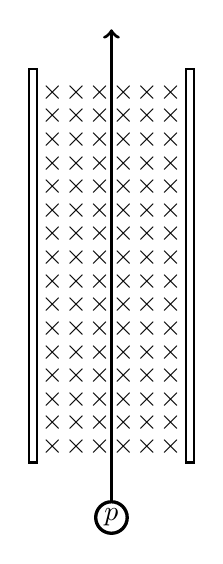
\begin{tikzpicture}
      \begin{scope}[thick]
        \draw(0,0) rectangle(.1,5);
          \draw(2,0) rectangle(2.1,5);
          \foreach\x in {.3,.6,...,2}{
            \foreach\y in {.2,.5,...,5} \node at (\x,\y) {$\times$};
          }
          \draw[very thick,->](1.05,-.5)--(1.05,5.5);
          \draw[very thick](1.05,-.7) circle(.2) node{$p$};
        \end{scope}
      \end{tikzpicture}
  \end{minipage}
  \begin{minipage}{.5\linewidth}
    \begin{choices}
      \choice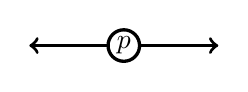
\begin{tikzpicture}
      \draw[very thick](0,0) circle(.2) node{$p$};
      \draw[very thick,->](.2,0)--(1.2,0);
      \draw[very thick,->](-.2,0)--(-1.2,0);
      \end{tikzpicture}

      \choice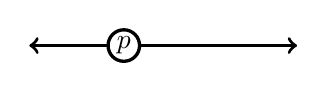
\begin{tikzpicture}
      \draw[very thick](0,0) circle(.2) node{$p$};
      \draw[very thick,->](.2,0)--(2.2,0);
      \draw[very thick,->](-.2,0)--(-1.2,0);
      \end{tikzpicture}
      
      \choice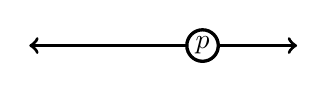
\begin{tikzpicture}
      \draw[very thick](0,0) circle(.2) node{$p$};
      \draw[very thick,->](.2,0)--(1.2,0);
      \draw[very thick,->](-.2,0)--(-2.2,0);
      \end{tikzpicture}

      \choice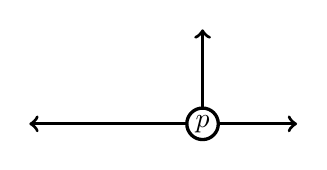
\begin{tikzpicture}
      \draw[very thick](0,0) circle(.2) node{$p$};
      \draw[very thick,->](.2,0)--(1.2,0);
      \draw[very thick,->](-.2,0)--(-2.2,0);
      \draw[very thick,->](0,.2)--(0,1.2);
      \end{tikzpicture}
    \end{choices}
  \end{minipage}
%    \columnbreak
%    
  \question Which of the following is true concerning the force on the
  current-carrying wire due to the electron?

  \begin{minipage}{.15\linewidth}
    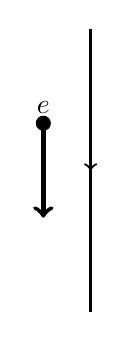
\begin{tikzpicture}[scale=1.2]
      \draw[thick,->](0,4)--(0,2.5);
      \draw[thick](0,2.52)--(0,1);
      \fill(-.5,3) circle(.08) node[above] {$e$};
      \draw[ultra thick,->](-.5,3)--(-.5,2) node[below]{$\varv$};
    \end{tikzpicture}
  \end{minipage}
  \begin{minipage}{.6\linewidth}
    \begin{choices}
      \choice The force is directed toward the right.
      \choice The force is directed toward the left.
      \choice The force is directed into the page.
    \choice There is no force on the current-carrying wire due to the electron.
    \end{choices}
  \end{minipage}

  \uplevel{
    \textbf{Questions \ref{q:2wires1}--\ref{q:2wires2}}
  
    Two wires carry currents $2A$ and $4A$ in the directions shown. Point $P$
    is a distance $r$ from the wire carrying $2A$, and a distance $2r$ from the
    wire carrying $4A$.
    \begin{center}
      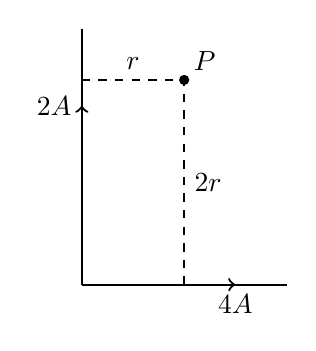
\begin{tikzpicture}[scale=1.3]
        \draw[thick](0,0)--(2,0);
        \draw[thick,->](0,0)--(1.5,0) node[below]{$4A$};
        \draw[thick](0,0)--(0,2.5);
        \draw[thick,->](0,0)--(0,1.75) node[left]{$2A$};
        \draw[thick,dashed](0,2)--(1,2)node[midway,above]{$r$}
        --(1,0) node[midway,right]{$2r$};
        \fill[black](1,2) circle(.05) node[above right]{$P$};
      \end{tikzpicture}
    \end{center}
  }

  \question Which of the following statements is true?
  \begin{choices}
    \choice The magnetic field produced at point $P$ by the wire carrying $2A$
    is greater than the magnetic field produced at point $P$ by the wire
    carrying $4A$, but opposite in direction.
    \choice The magnetic field produced at point $P$ by the wire carrying $2A$
    is less than the magnetic field produced at point $P$ by the wire
    carrying $4A$, and in the same direction.
    \choice The magnetic field produced at point $P$ by the wire carrying $2A$
    is equal to the magnetic field produced at point $P$ by the wire
    carrying $4A$, but opposite in direction.
    \choice The magnetic field produced at point $P$ by the wire carrying $2A$
    is equal to the magnetic field produced at point $P$ by the wire
    carrying $4A$, and in the same direction.
    \choice The magnetic field produced at point $P$ by the wire carrying $2A$
    is greater than the magnetic field produced at point $P$ by the wire
    carrying $4A$, and in the same direction.
  \end{choices}
  \label{q:2wires1}
    
  \question The magnitude of the resultant magnetic field at point $P$ due to
  the current in the two wires is
  \begin{choices}
    \choice zero
    \choice $\dfrac{\mu_0(2A)}{2\pi r}$
    \choice $\dfrac{\mu_0(2A)}{\pi r}$
    \choice $\dfrac{\mu_0(4A)}{2\pi r}$
    \choice $\dfrac{\mu_0(6A)}{4\pi r}$
    \end{choices}
  \label{q:2wires2}

%  \end{enumerate}
%  \columnbreak
  \uplevel{
    \textbf{Questions \ref{q:2curr1}--\ref{q:2curr2}}

    Two wires are parallel to each other, one carrying twice the current as the
    other. The two currents flow in the same direction.
  }

  \question Which of the following is true of the forces the wires exert on each
  other?
  \begin{choices}
    \choice The wire with the larger current exerts a greater force on the other
    wire.
    \choice The wire with the smaller current exerts a greater force on the
    other wire.
    \choice The wires exert equal and opposite forces on each other.
    \choice The wires exert equal forces on each other, but in the same
    direction.
    \choice The net force between the wires is zero.
  \end{choices}
  \label{q:2curr1}
    
  \question The direction of the force between the wires is
  \begin{choices}
    \choice repulsive
    \choice attractive
    \choice zero
    \choice into the page
    \choice out of the page
  \end{choices}
  \label{q:2curr2}
    
  \question A loop of wire in the plane of the page carries a clockwise current
  $I$ and is placed in a magnetic field that is directed into the page as shown.
  Which of the following will happen as a result of the wire loop being in
  the magnetic field?
  
  \begin{minipage}{.25\linewidth}
    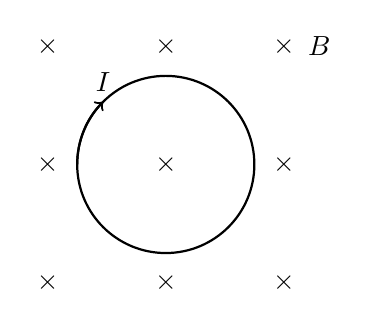
\begin{tikzpicture}[scale=1.5]
      \foreach \x in {-1,0,1}{
        \foreach \y in {-1,0,1}{
          \node at (\x,\y) {$\bm\times$};
        }
      }
      \draw[thick](0,0) circle(.75);
      \draw[thick,->](-.75,0) arc(180:135:.75) node[above]{$I$};
      \node at (1.3,1) {$B$};
    \end{tikzpicture}
  \end{minipage}
  \begin{minipage}{.5\linewidth}
    \begin{choices}
      \choice The wire loop will rotate clockwise.
      \choice The wire loop will rotate counterclockwise.
      \choice The wire loop will flip on a horizontal axis through its center.
      \choice The wire loop will expand in size.
      \choice The wire loop will contract in size.
    \end{choices}
  \end{minipage}
  \vspace{.2in}

  \newpage
  
  \uplevel{
    \textbf{Questions \ref{q:circ1}--\ref{q:circ2}}
    
    A negatively charged particle of mass $m$ and charge $q$ in a uniform
    magnetic field $B$ travels in a circular path of radius $r$.
    \begin{center}
      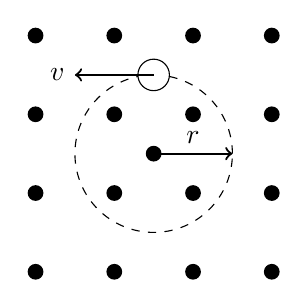
\begin{tikzpicture}
        \foreach \x in {0,...,3}{
        \foreach \y in {0,...,3}{
          \fill[black](\x,\y)circle(.1);
        }
        }
        \fill[black](1.5,1.5)circle(.1);
        \draw[thick,->](1.5,1.5)--(2.5,1.5) node[midway,above]{$r$};
        \draw[dashed](1.5,1.5) circle(1);
        \draw[fill=white](1.5,2.5) circle(.2);
        \draw[thick,->](1.5,2.5)--(.5,2.5) node[left]{$v$};
      \end{tikzpicture}
    \end{center}
  }
  
  \question In terms of the other given quantities, the charge-to-mass ratio
  $q/m$ of the particle is
  \begin{choices}
    \choice $\dfrac{Bv}{r}$
    \choice $\dfrac{r}{Bv}$
    \choice $\dfrac{rv}{B}$
    \choice $rvB$
    \choice $\dfrac{v}{rB}$
  \end{choices}
  \label{q:circ1}
    
  \question The work done by the magnetic field after two full revolutions of
  the charge is
  \begin{choices}
    \choice zero
    \choice $-qvB/rm$
    \choice $qvm/Br$
    \choice $-mBr/qv$
    \choice $-mqvBr$
  \end{choices}
  \label{q:circ2}
%    \columnbreak
%    
  \question A dynamic microphone contains a magnet and a coil of wire connected
  toa movable diaphragm, as shown in the figure. Sound waves directed at the
  diaphragm generate a current in the wires leading from the coil. Which of
  the following helps to explain why this occurs?

  \begin{minipage}{.5\linewidth}
    \pic{.9}{mic}
  \end{minipage}
  \begin{minipage}{.49\linewidth}
    \begin{choices}
      \choice The area of the coil changes.
      \choice The magnitude of the magnetic field produced by the magnet
      changes.
      \choice The angle between the plane of the coil and the magnetic field
      produced by the magnet change.
      \choice The strength of the magnetic field in the plane of the coil
      changes.
    \end{choices}
  \end{minipage}

  \question A current is passed through an analog ammeter and the needle moves
  to indicate the current flowing through the circuit. Which of the
  following best explains how an analog ammeter works?
  \begin{choices}
    \choice Current is passed through the needle placed in a magnetic field,
    and the needle is attracted to the high side of the scale.
    \choice The needle is a magnet, and is attracted to a magnet on the high
    side of the scale.
    \choice The needle gathers an electrostatic charge from the current, and is
    attracted to an electrostatic charge on the high side of the scale.
    \choice Current is passed through a spring coil of wire placed in a
    magnetic field, and the coil rotates, moving the needle
    proportionally to the current in the coil.
    \choice Current flows through the needle, making it heavier, and it falls to
    the high side of the scale.
  \end{choices}
  \vspace{.7in}
    
  \question An electric motor consists of a current-carrying loop of wire
  mounted to an axle and turned at a slight angle in a magnetic field as shown.
  The wire loop will
  \begin{center}
    \pic{.35}{motor-drawing}
  \end{center}
  \begin{choices}
    \choice experience a torque and turn clockwise
    \choice experience a torque and turn counterclockwise
    \choice accelerate upward out of the magnetic field
    \choice accelerate downward out of the magnetic field
    \choice not experience a force or torque
  \end{choices}
  \newpage

  \uplevel{
    \centering
    \begin{tikzpicture}[american voltages,scale=1.4]
      \begin{scope}[thick]
        \draw(1.5,0)--(0,0) to[battery,l=$\mathcal{E}$] (0,2)--(1.5,2);
        \draw(1.5,1.9) rectangle(8,2.1);
        \draw(1.5,-.1) rectangle(8,.1);
        \draw[<->](7.5,.1)--(7.5,1.9) node[midway,left]{$d$};
        \draw(1.1,1) circle(.1) node[above]{$m$} node[below left]{$q$};
        \draw[->](1.2,1)--(2,1) node[right]{$\varv$};
      \end{scope}
    \end{tikzpicture}
  }

  \question A positively charged particle ($q$) of mass $m$ travels
  horizontally, with a velocity of $\varv$, through the center of two capacitor
  plates. The plates areseparated by a distance of $d$ and connected to a
  battery of potential difference ($\mathcal{E}$), as shown in the figure.
  \begin{parts}
    \part Sketch the electric field between the plates.
    \part Derive an algebraic expression for the electric field between the
    plates in terms of given quantities. Show all your work.
    \part Describe the motion of the particle as it passes through the capacitor
    plates. What shape is the path? Which direction is the acceleration?
    \part What direction of magnetic field is needed to make the particle travel
    horizontally straight through the capacitor plates?
    \part Derive an algebraic expression for the magnitude of the magnetic field
    needed to cause this straight, horizontal motion between the plates in
    terms of given quantities. Show all your work.
    \part The crossed electric and magnetic fields are adjusted to cause
    positively charged particles with a velocity of vto travel straight. What
    happens to a particle traveling at $2\varv$? Will it travel straight, or
    will it curve? If it curves, indicate which way it will curve, and explain
    why. If it continues to travel straight, explain why.
    \part The crossed electric and magnetic fields are tuned to cause positively
    charged particles with a velocity of vto travel straight. What happens
    to a negatively charged particle traveling at v? Will it travel straight, or
    will it curve? If it curves, indicate which way it will curve, and explain
    why. If is continues to travel straight, explain why.
  \end{parts}
  \newpage

  \uplevel{
    \centering
    \begin{tikzpicture}
      \foreach\x in {0,...,5}{
        \foreach\y in {0,...,5}\fill(\x,\y) circle(.1);
      }
      \draw[thick](6,.5) --(-2,.5) to[R,l=$R$] (-2,4.3)--(6,4.3);
      \draw[thick,<->](5.7,.5)--(5.7,4.3) node[midway,right]{$y$};
      \fill(1.4,0.3) rectangle(1.6,4.6);
      \draw[very thick,->](.5,2.5)--(3.8,2.5) node[right]{$\varv$};
      \draw[thick,<->](-2,-.3)--(1.5,-.3) node[midway,below]{$x$};
      \node at(4.5,5.4){$B$};
    \end{tikzpicture}
  }
  \question Two long parallel wires, separated by a distance of $y$, pass
  through a region of magnetic field ($B$). The two wires are connected by a
  resistor ($R$) and a metal bar, separated by a distance of $x$, to produce a
  circuit loop, as shown in the figure. The metal bar slides along the wires to
  the right at a velocity of $\varv$.
  \begin{parts}
    \part Calculate the induced emf ($e$) in the bar in terms of the given
    quantities.
    \part Calculate the current in the circuit in terms of the given quantities.
    \part What is the direction of the current in the resistor--upward or
    downward?
  \end{parts}
  \newpage

  % TAKEN FROM 2003 AP PHYSICS B EXAM FREE-RESPONSE QUESTION 3
  \uplevel{
    \cpic{.7}{magnetic}
  }
  \question A rail gun is a device that propels a projectile using a magnetic
  force. A simplified diagram of this device is shown above. The projectile in
  the picture is a bar of mass $M$ and length $D$, which has a constant current
  $I$ flowing through it in the $+y$-direction, as shown. The space between the
  thin frictionless rails contains a uniform magnetic field $\bm{B}$,
  perpendicular to the plane of the page. The magnetic field and rails extend
  for a distance $L$. The magnetic field exerts a constant force $\bm{F}$ on
  the projectile, as shown.

  Express all algebraic answers to the following parts in terms of the
  magnitude $F$ of the constant magnetic force, other quantities given above,
  and fundamental constants.
  \begin{parts}
    \part Determine the position $x$ of the projectile as a function of time $t$
    while it is on the rail if the projectile starts from rest at $x=0$ when
    $t=0$.
    
    \part Determine the speed of the projectile as it leaves the right-hand end
    of the track.
    
    \part Determine the energy supplied to the projectile by the rail gun.

    \part In what direction must the magnetic field $\bm{B}$ point in order to
    create the force $\bm{F}$? Explain your reasoning.

    \part Calculate the speed of the bar when it reaches the end of the rail
    given the following values.

    $B=\SI{5}{\tesla}$\hspace{.3in}
    $L=\SI{10}{\metre}$\hspace{.3in}
    $I=\SI{200}{\ampere}$\hspace{.3in}
    $M=\SI{.5}{\kilo\gram}$\hspace{.3in}
    $D=\SI{10}{\centi\metre}$
  \end{parts}
  \newpage

  
  % TAKEN FROM THE 2008 AP PHYSICS B FREE-RESPONSE QUESTION #3
  \question A rectangular wire loop is connected across a power supply with an
  internal resistance of \SI{.50}{\ohm} and an emf of \SI{16}{\volt}. The wire
  has resistivity \SI{1.7e-8}{\ohm\metre} and cross-sectional area
  \SI{3.5e-9}{\metre\squared}. When the power supply is turned on, the current
  in the wire is \SI{4.}{\ampere}.
  \begin{parts}
    \part Calculate the length of wire used to make the loop.
%  \end{enumerate}
    \uplevel{
      The wire loop is then used in an experiment to measure the strength of
      the magnetic field between the poles of a magnet. The magnet is placed on
      a digital balance, and the wire loop is held fixed between the poles of
      the magnet, as shown below. The \SI{.020}{\metre} long horizontal segment
      of the loop is midway between the poles and perpendicular to the
      direction of the magnetic field. The power supply in the loop is turned
      on, so that the \SI{4.}{\ampere} current is in the direction shown.
      \begin{center}
        \pic{.4}{current-magnet}
        
        \underline{Note:} Figure not drawn to scale.
      \end{center}
    }

    \part In which direction is the force on the magnet due to the current in
    the wire segment? Justify your answer.

    \vspace{.1in}
    \underline{\hspace{.4in}} Upward\hspace{.5in}
    \underline{\hspace{.4in}} Downward

    \part The reading on the balance changed by \SI{.060}{\newton} when the
    power supply was turned on. Calculate the strength of the magnetic field.

    \newpage
    \uplevel{
      Suppose that various rectangular loops with the same total length of wire
      as found in part (a) were constructed such that the lengths of the
      horizontal segments of the wire loops varied between 0.02 m and 0.10 m.
      The horizontal segment of each loop was always centered between the
      poles, and the current in each loop was always 4.0 A. The following graph
      represents the theoretical relationship between the magnitude of the
      force on the magnet and the length of the wire.
      \begin{center}
        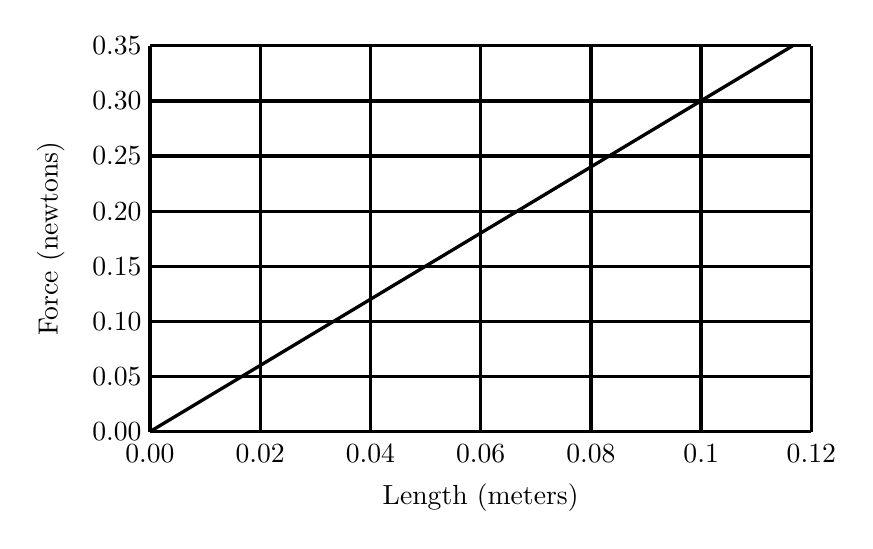
\begin{tikzpicture}[xscale=1.4,yscale=.7]
          \draw[very thick](0,0) grid(6,7);
          \foreach\x in {0.00,0.02,0.04,0.06,0.08,0.1,0.12}
          \node at (\x*50,-.4){\x};
          \node at (3,-1.2){Length (meters)};
      
          \foreach\y in {0.00,0.05,0.10,0.15,0.20,0.25,0.30,0.35}
          \node at (-.3,\y*20){\y};
          \node[rotate=90] at (-.9,3.5){Force (newtons)};
          \draw[very thick](0,0)--(5.83,7);
        \end{tikzpicture}
      \end{center}
    }

    \part On the graph above, sketch a possible relationship between the
    magnitude of the force on the magnet and the length of the wire segment if
    the wire segments were misaligned and placed at a constant nonperpendicular
    angle to the magnetic field, as shown below.
    \begin{center}
      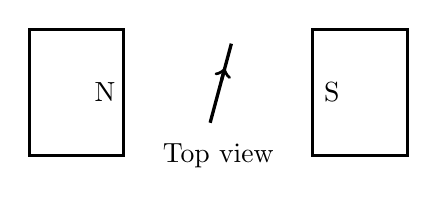
\begin{tikzpicture}[scale=.8]
        \draw[very thick](1.5,-1) rectangle(3,1);
        \draw[very thick](-1.5,-1) rectangle(-3,1);
        \node at (1.8,0) {S};
        \node at (-1.8,0){N};
        \node at (0,-1){Top view};
        \begin{scope}[rotate=-15]
          \draw[very thick,->](0,-.5)--(0,.4);
          \draw[very thick](0,.2)--(0,.8);
        \end{scope}
      \end{tikzpicture}
    \end{center}
    
    \part Suppose the loops are correctly placed perpendicular to the field and
    the following data are obtained. Describe a likely cause of the discrepancy
    between the data and the theoretical relationship.
    \begin{center}
      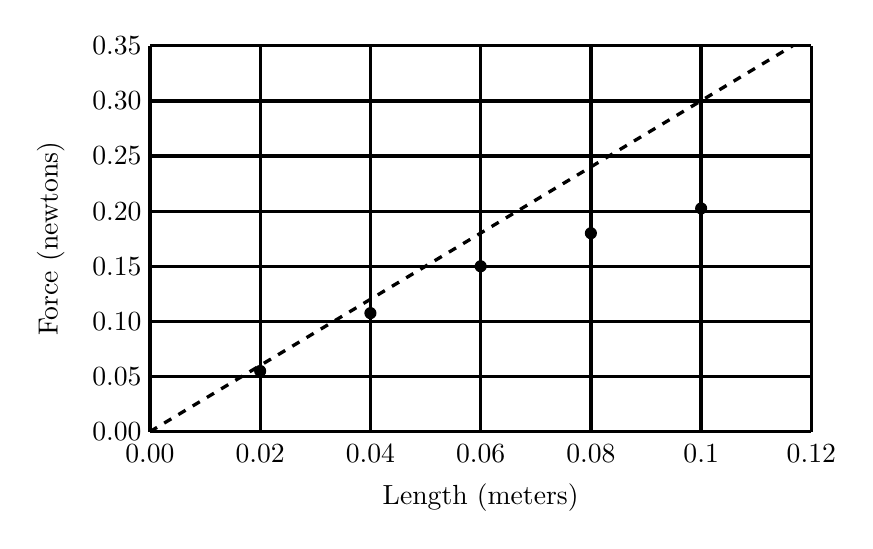
\begin{tikzpicture}[xscale=1.4,yscale=.7]
        \draw[very thick](0,0) grid(6,7);
        \foreach\x in {0.00,0.02,0.04,0.06,0.08,0.1,0.12}
        \node at (\x*50,-.4){\x};
        \node at (3,-1.2){Length (meters)};
      
        \foreach\y in {0.00,0.05,0.10,0.15,0.20,0.25,0.30,0.35}
        \node at (-.3,\y*20){\y};
        \node[rotate=90] at (-.9,3.5){Force (newtons)};

        \draw[very thick,dashed](0,0)--(5.83,7);
        \fill(1,1.1) circle(.055 and .11);
        \fill(2,2.15)circle(.055 and .11);
        \fill(3,3)   circle(.055 and .11);
        \fill(4,3.6) circle(.055 and .11);
        \fill(5,4.05)circle(.055 and .11);
      \end{tikzpicture}
    \end{center}
  \end{parts}
  \newpage
  
  % TAKEN FROM 2014 AP PHYSICS B FREE-RESPONSE QUESTION #5
  \uplevel{
    \cpic{.6}{battery-magfield}
  }
  \question A conducting rod of mass $m$ and length $L$ hangs at rest from two
  identical conducting springs, each with spring constant $k$, as shown in the
  figure at left above. The upper ends of the springs are fixed at points $P$
  and $Q$, and the rod is in a uniform magnetic field $\bm{B}$ directed into
  the page. A battery is then connected between points $P$ and $Q$, as shown in
  the figure at right above, resulting in a current $I$ in the rod. The rod is
  displaced downward, eventually reaching a new equilibrium position with the
  springs stretched an additional distance $\Delta y$.

  \begin{parts}
    \part Which point, $P$ or $Q$, is connected to the positive terminal of the
    battery? Justify your answer.

    \underline{\hspace{.5in}} P\hspace{.3in}
    \underline{\hspace{.5in}} Q
        
    \part On the dot below that represents the rod, draw and label the forces
    (not components) that act on the rod in its new equilibrium position. Each
    force must be represented by a distinct arrow starting on, and pointing away
    from, the dot.

    \vspace{.4in}
    \begin{center}
      
\begin{tikzpicture}
        \fill(0,0) circle(.18);
      \end{tikzpicture}
    \end{center}
    \vspace{.4in}
    
    \part Derive an expression for $\Delta y$ in terms of $k$, $m$, $L$, $I$,
    the magnetic field strength $B$, and fundamental constants, as appropriate.
    \newpage

    \uplevel{
      An experiment is conducted with batteries of different emf connected
      between points $P$ and $Q$. The current $I$ in the rod and the stretch of
      the springs $\Delta y$ are measured and recorded in the table below.
      \begin{center}
        \begin{tabular}{|c|c|}
          \hline
          $I$ (amperes) & $\Delta y$ (meters)\\\hline
          1.0 & 0.0028\\\hline
          2.0 & 0.0050\\\hline
          3.0 & 0.0084\\\hline
          4.0 & 0.0119\\\hline
          5.0 & 0.0140\\\hline
        \end{tabular}
      \end{center}
    }

    \part On the grid below, plot the data points for $\Delta y$ as a function
    of $I$. Be sure to label your axes with variables, units, and scale. Draw a
    straight line that best represents the data.
    
    \vspace{.2in}
    \begin{center}
      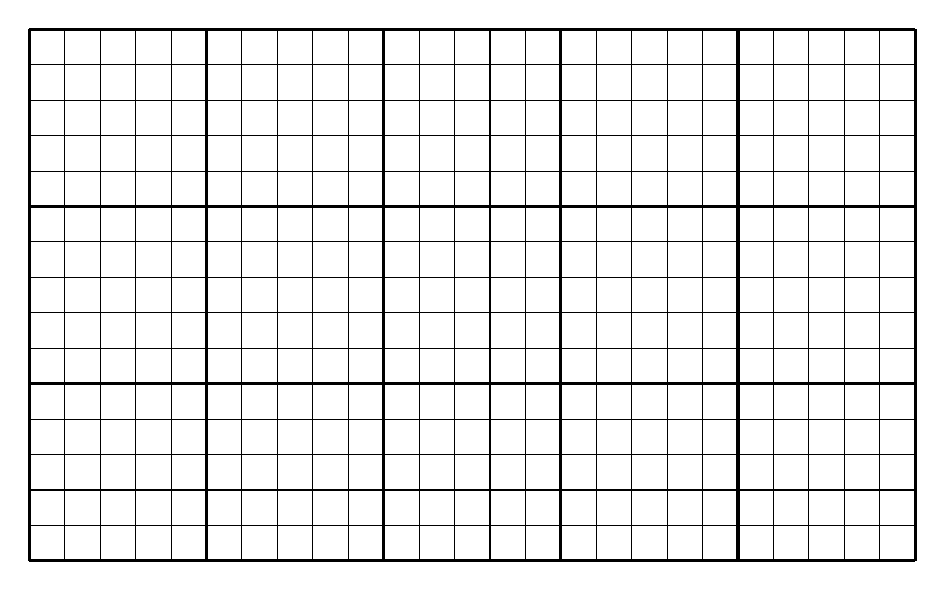
\begin{tikzpicture}[scale=.45]
        \draw(0,0) grid (25,15);
        \foreach \x in {0,5,...,25}\draw[very thick](\x,0)--(\x,15);
        \foreach \y in {0,5,10,15} \draw[very thick](0,\y)--(25,\y);
      \end{tikzpicture}
    \end{center}
    \vspace{.3in}
    
    \part Using the straight line you drew in part (d), calculate the value $B$
    for the magnetic field if $m$ is \SI{.019}{\kilo\gram}, $L$ is
    \SI{.35}{\metre}, and $k$ is \SI{25}{\newton\per\metre}.
  \end{parts}
\end{questions}
\end{document}
